% Diagrama A — pipeline experimental com as três condições e teste real comum.
\documentclass[tikz,border=6pt]{standalone}
% Preâmbulo compartilhado dos diagramas conceituais do relatório CoInfoSim.
% Compilação: xelatex (determinística; nenhum dado experimental é usado).
\usepackage{fontspec}
\setmainfont{Liberation Sans}
\setsansfont{Liberation Sans}
\usepackage{amsmath}
\usepackage{bm}
\usepackage{tikz}
\usetikzlibrary{arrows.meta,positioning,calc,fit,backgrounds,decorations.pathreplacing,matrix,patterns}
\definecolor{CoinAccent}{RGB}{25,80,140}
\definecolor{CoinAccentDark}{RGB}{18,55,95}
\definecolor{CoinAccentPale}{RGB}{237,242,248}
\definecolor{CoinGray}{RGB}{95,95,95}
\definecolor{CoinGrayPale}{RGB}{246,246,246}
\definecolor{CoinWin}{RGB}{76,140,90}    % verde discreto (vitória)
\definecolor{CoinLose}{RGB}{182,88,79}   % vermelho discreto (derrota)
\tikzset{
  bloco/.style={draw=CoinAccentDark, fill=CoinAccentPale, rounded corners=1.2pt,
                align=center, font=\small, inner sep=4pt, minimum height=7mm},
  bloconeutro/.style={draw=CoinGray, fill=CoinGrayPale, rounded corners=1.2pt,
                align=center, font=\small, inner sep=4pt, minimum height=7mm},
  blocoreal/.style={draw=CoinAccentDark, fill=white, rounded corners=1.2pt,
                align=center, font=\small, inner sep=4pt, minimum height=7mm},
  seta/.style={-{Stealth[length=2.4mm]}, thick, CoinAccentDark},
  setacinza/.style={-{Stealth[length=2.4mm]}, thick, CoinGray},
  rotulo/.style={font=\footnotesize\itshape, text=CoinGray, align=center},
}

\begin{document}
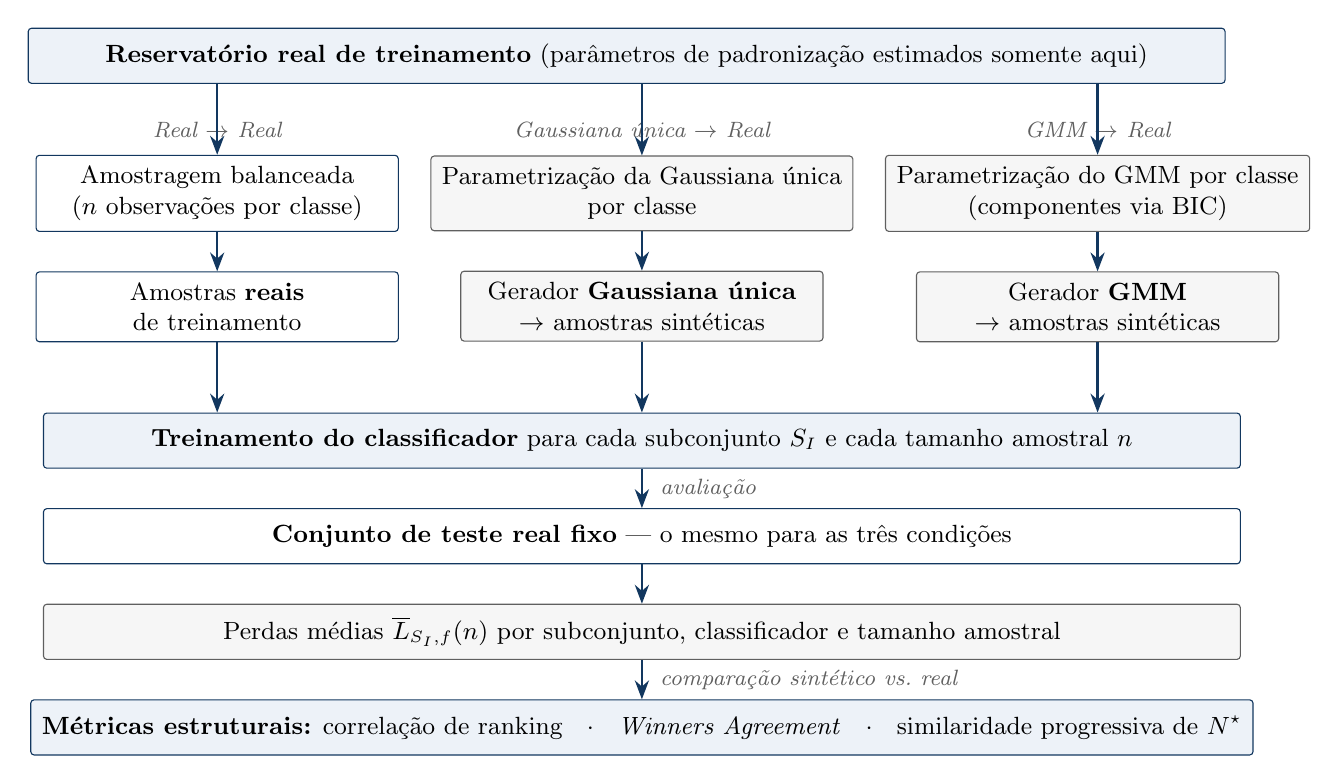
\begin{tikzpicture}[node distance=5mm and 7mm]
  % Reservatório real
  \node[bloco, minimum width=15.2cm] (reserv)
    {\textbf{Reservatório real de treinamento} (parâmetros de padronização estimados somente aqui)};

  % Colunas: real / gaussiana / gmm
  \node[blocoreal, below=9mm of reserv.south west, anchor=north west, xshift=1mm,
        minimum width=4.6cm] (amostraReal)
    {Amostragem balanceada\\($n$ observações por classe)};
  \node[bloconeutro, right=4mm of amostraReal, minimum width=4.6cm] (estGauss)
    {Parametrização da Gaussiana única\\por classe};
  \node[bloconeutro, right=4mm of estGauss, minimum width=4.6cm] (estGmm)
    {Parametrização do GMM por classe\\(componentes via BIC)};

  \node[blocoreal, below=of amostraReal, minimum width=4.6cm] (treinoReal)
    {Amostras \textbf{reais}\\de treinamento};
  \node[bloconeutro, below=of estGauss, minimum width=4.6cm] (gerGauss)
    {Gerador \textbf{Gaussiana única}\\$\rightarrow$ amostras sintéticas};
  \node[bloconeutro, below=of estGmm, minimum width=4.6cm] (gerGmm)
    {Gerador \textbf{GMM}\\$\rightarrow$ amostras sintéticas};

  % Rótulos das condições
  \node[rotulo, above=1mm of amostraReal] {Real $\rightarrow$ Real};
  \node[rotulo, above=1mm of estGauss] {Gaussiana única $\rightarrow$ Real};
  \node[rotulo, above=1mm of estGmm] {GMM $\rightarrow$ Real};

  % Treinamento e avaliação comuns
  \node[bloco, below=9mm of gerGauss, minimum width=15.2cm] (clf)
    {\textbf{Treinamento do classificador} para cada subconjunto $S_I$ e cada tamanho amostral $n$};
  \node[bloco, below=of clf, minimum width=15.2cm, fill=white] (teste)
    {\textbf{Conjunto de teste real fixo} --- o mesmo para as três condições};
  \node[bloconeutro, below=of teste, minimum width=15.2cm] (perdas)
    {Perdas médias $\overline{L}_{S_I,f}(n)$ por subconjunto, classificador e tamanho amostral};
  \node[bloco, below=of perdas, minimum width=15.2cm] (metricas)
    {\textbf{Métricas estruturais:} correlação de ranking \; $\cdot$ \; \textit{Winners Agreement} \; $\cdot$ \; similaridade progressiva de $N^{\star}$};

  % Setas
  \draw[seta] (reserv.south -| amostraReal) -- (amostraReal.north);
  \draw[seta] (reserv.south -| estGauss) -- (estGauss.north);
  \draw[seta] (reserv.south -| estGmm) -- (estGmm.north);
  \draw[seta] (amostraReal) -- (treinoReal);
  \draw[seta] (estGauss) -- (gerGauss);
  \draw[seta] (estGmm) -- (gerGmm);
  \draw[seta] (treinoReal.south) -- (clf.north -| treinoReal);
  \draw[seta] (gerGauss.south) -- (clf.north -| gerGauss);
  \draw[seta] (gerGmm.south) -- (clf.north -| gerGmm);
  \draw[seta] (clf) -- node[right=1mm, rotulo] {avaliação} (teste);
  \draw[seta] (teste) -- (perdas);
  \draw[seta] (perdas) -- node[right=1mm, rotulo] {comparação sintético vs.\ real} (metricas);
\end{tikzpicture}
\end{document}
